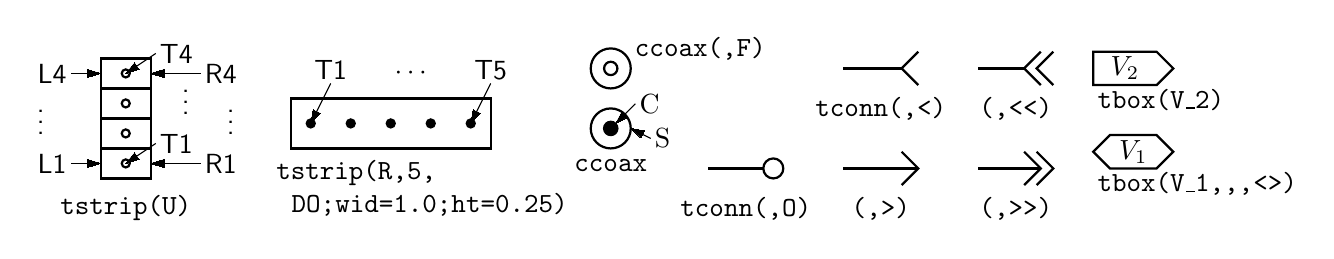
\begin{tikzpicture}[scale=2.54]
% dpic version 2020.03.01 option -g for TikZ and PGF 1.01
\ifx\dpiclw\undefined\newdimen\dpiclw\fi
\global\def\dpicdraw{\draw[line width=\dpiclw]}
\global\def\dpicstop{;}
\dpiclw=0.8bp
\dpiclw=0.8bp
{\sf
\global\let\dpicshdraw=\dpicdraw\global\def\dpicdraw{}
\global\def\dpicstop{--}
\dpicshdraw[fill=white!100!black]
\dpicdraw (0.502778,0.324448)
 --(0.377778,0.324448)
 --(0.377778,-0.275552)
 --(0.627778,-0.275552)
 --(0.627778,0.324448)
 --(0.502778,0.324448)\dpicstop
cycle; \global\let\dpicdraw=\dpicshdraw\global\def\dpicstop{;}
\dpicdraw (0.627778,-0.125552)
 --(0.377778,-0.125552)\dpicstop
\dpicdraw (0.627778,0.024448)
 --(0.377778,0.024448)\dpicstop
\dpicdraw (0.627778,0.174448)
 --(0.377778,0.174448)\dpicstop
\dpicdraw[fill=white](0.502778,-0.200552) circle (0.007874in)\dpicstop
\dpicdraw[fill=white](0.502778,-0.050552) circle (0.007874in)\dpicstop
\dpicdraw[fill=white](0.502778,0.099448) circle (0.007874in)\dpicstop
\dpicdraw[fill=white](0.502778,0.249448) circle (0.007874in)\dpicstop
\dpiclw=0.4bp
\filldraw[line width=0bp](0.311111,-0.220552)
 --(0.377778,-0.200552)
 --(0.311111,-0.180552) --cycle\dpicstop
\dpicdraw (0.368111,-0.200552)
 --(0.227778,-0.200552)\dpicstop
\draw (0.227778,-0.200552) node[left=-2bp]{L1};
\filldraw[line width=0bp](0.311111,0.229448)
 --(0.377778,0.249448)
 --(0.311111,0.269448) --cycle\dpicstop
\dpicdraw (0.368111,0.249448)
 --(0.227778,0.249448)\dpicstop
\draw (0.227778,0.249448) node[left=-2bp]{L4};
\draw (0.077778,0.044448) node{$\vdots$};
\filldraw[line width=0bp](0.694444,-0.180552)
 --(0.627778,-0.200552)
 --(0.694444,-0.220552) --cycle\dpicstop
\dpicdraw (0.637445,-0.200552)
 --(0.877778,-0.200552)\dpicstop
\draw (0.877778,-0.200552) node[right=-2bp]{R1};
\filldraw[line width=0bp](0.694444,0.269448)
 --(0.627778,0.249448)
 --(0.694444,0.229448) --cycle\dpicstop
\dpicdraw (0.637445,0.249448)
 --(0.877778,0.249448)\dpicstop
\draw (0.877778,0.249448) node[right=-2bp]{R4};
\draw (1.027778,0.044448) node{$\vdots$};
\filldraw[line width=0bp](0.547154,-0.146931)
 --(0.502778,-0.200552)
 --(0.569342,-0.180213) --cycle\dpicstop
\dpicdraw (0.510821,-0.195189)
 --(0.652778,-0.100552)\dpicstop
\draw (0.652778,-0.100552) node[right=-2bp]{T1};
\filldraw[line width=0bp](0.547154,0.303069)
 --(0.502778,0.249448)
 --(0.569342,0.269787) --cycle\dpicstop
\dpicdraw (0.510821,0.254811)
 --(0.652778,0.349448)\dpicstop
\draw (0.652778,0.349448) node[right=-2bp]{T4};
\draw (0.802778,0.144448) node{$\vdots$};
\dpiclw=0.8bp
\draw (0.502778,-0.425552) node(CS1){\tt tstrip(U)};
\global\let\dpicshdraw=\dpicdraw\global\def\dpicdraw{}
\global\def\dpicstop{--}
\dpicshdraw[fill=white!100!black]
\dpicdraw (2.327778,-0.000552)
 --(2.327778,0.124448)
 --(1.327778,0.124448)
 --(1.327778,-0.125552)
 --(2.327778,-0.125552)
 --(2.327778,-0.000552)\dpicstop
cycle; \global\let\dpicdraw=\dpicshdraw\global\def\dpicstop{;}
\dpicdraw[fill=black](1.427778,-0.000552) circle (0.007874in)\dpicstop
\dpicdraw[fill=black](1.627778,-0.000552) circle (0.007874in)\dpicstop
\dpicdraw[fill=black](1.827778,-0.000552) circle (0.007874in)\dpicstop
\dpicdraw[fill=black](2.027778,-0.000552) circle (0.007874in)\dpicstop
\dpicdraw[fill=black](2.227778,-0.000552) circle (0.007874in)\dpicstop
\dpiclw=0.4bp
\filldraw[line width=0bp](1.439703,0.068021)
 --(1.427778,-0.000552)
 --(1.475481,0.050132) --cycle\dpicstop
\dpicdraw (1.432101,0.008095)
 --(1.527778,0.199448)\dpicstop
\draw (1.527778,0.199448) node[above=-2bp]{T1};
\filldraw[line width=0bp](2.239703,0.068021)
 --(2.227778,-0.000552)
 --(2.275481,0.050132) --cycle\dpicstop
\dpicdraw (2.232101,0.008095)
 --(2.327778,0.199448)\dpicstop
\draw (2.327778,0.199448) node[above=-2bp]{T5};
\draw (1.927778,0.199448) node[above=-2bp]{$\cdots$};
\draw (1.227778,-0.325552) node(CS2){\shortstack{\rlap{\hbox to 2bp{}\tt tstrip(R,5,}\\%
\rlap{\hbox to 2bp{}\tt $\;\;$DO;wid=1.0;ht=0.25)}}};
}
\dpiclw=0.8bp
\dpicdraw (2.927778,-0.025552) circle (0.03937in)\dpicstop
\dpicdraw[fill=black](2.927778,-0.025552) circle (0.013123in)\dpicstop
\draw (2.927778,-0.125552) node[below=-2bp]{\tt ccoax\vphantom{(}};
\dpiclw=0.4bp
\filldraw[line width=0bp](2.984346,0.059301)
 --(2.951348,-0.001982)
 --(3.012631,0.031017) --cycle\dpicstop
\dpicdraw (2.965019,0.01169)
 --(3.051348,0.098018)\dpicstop
\draw (3.051348,0.098018) node[right=-2bp]{C};
\filldraw[line width=0bp](3.096351,-0.037477)
 --(3.027778,-0.025552)
 --(3.078462,-0.073255) --cycle\dpicstop
\dpicdraw (3.045071,-0.034198)
 --(3.127778,-0.075552)\dpicstop
\draw (3.127778,-0.075552) node[right=-2bp]{S};
\dpiclw=0.8bp
\dpicdraw (2.927778,0.274448) circle (0.03937in)\dpicstop
\dpicdraw[fill=white](2.927778,0.274448) circle (0.013123in)\dpicstop
\draw (3.027778,0.374448) node[right=-2bp]{\tt ccoax(,F)};
\dpicdraw (3.740551,-0.225552) circle (0.019685in)\dpicstop
\dpicdraw (3.415551,-0.225552)
 --(3.690551,-0.225552)\dpicstop
\draw (3.603051,-0.425552) node{\tt tconn(,O)};
\dpicdraw (4.090551,-0.225552)
 --(4.465551,-0.225552)\dpicstop
\dpicdraw (4.382218,-0.142218)
 --(4.465551,-0.225552)
 --(4.382218,-0.308885)\dpicstop
\draw (4.278051,-0.425552) node{\tt (,>)};
\dpicdraw (4.765551,-0.225552)
 --(5.078051,-0.225552)\dpicstop
\dpicdraw (4.994718,-0.142218)
 --(5.078051,-0.225552)
 --(4.994718,-0.308885)\dpicstop
\dpicdraw (5.057218,-0.142218)
 --(5.140551,-0.225552)
 --(5.057218,-0.308885)\dpicstop
\draw (4.953051,-0.425552) node{\tt (,>>)};
\dpicdraw (4.090551,0.274448)
 --(4.382218,0.274448)\dpicstop
\dpicdraw (4.465551,0.357782)
 --(4.382218,0.274448)
 --(4.465551,0.191115)\dpicstop
\draw (4.278051,0.074448) node{\tt tconn(,<)};
\dpicdraw (4.765551,0.274448)
 --(4.994718,0.274448)\dpicstop
\dpicdraw (5.078051,0.357782)
 --(4.994718,0.274448)
 --(5.078051,0.191115)\dpicstop
\dpicdraw (5.140551,0.357782)
 --(5.057218,0.274448)
 --(5.140551,0.191115)\dpicstop
\draw (4.953051,0.074448) node{\tt (,<<)};
\dpicdraw (5.540551,0.357782)
 --(5.657218,0.357782)
 --(5.740551,0.274448)
 --(5.657218,0.191115)
 --(5.340551,0.191115)
 --(5.340551,0.357782)
 --(5.540551,0.357782)\dpicstop
\draw (5.498884,0.274448) node{$ V_2$};
\draw (5.340551,0.191115) node[below right=-2bp]{\tt tbox(V\_2)};
\dpicdraw (5.540551,-0.225552)
 --(5.423884,-0.225552)
 --(5.340551,-0.142218)
 --(5.423884,-0.058885)
 --(5.657218,-0.058885)
 --(5.740551,-0.142218)
 --(5.657218,-0.225552)
 --(5.540551,-0.225552)\dpicstop
\draw (5.540551,-0.142218) node{$ V_1$};
\draw (5.340551,-0.225552) node[below right=-2bp]{\tt tbox(V\_1,{,},<>)};
\end{tikzpicture}
\vspace*{-0.5\baselineskip}
